\subsection*{Question}
Design a randomized non-preemptive algorithm which is $O(\log n)$ competitive.

\subsection*{Answer}
First of all, looking at the greedy algorithm in the bounded case for $\left[2^{i-1},2^i\right]$ , we want to understand what it's competitiveness is. In the worst case for a given request, we first have 2 edges that ON won't be able to take from (like in the normal case) which are on its edges (doesn't matter whether both edges are on the same line or a different one), now like in last section, we need to add 2 more paths that will be blocked because they were across edges. For example if $A$ is from $k_1^1$ to $k_2^1$ then the ones blocked are on either edges which are lines 1,2 of the star and any 2 which cross from a third line to line 1 and line 2, and there are at most 2 of those. Lastly we need to add the 2 possible paths that are between the first and third line and second and fourth line. Note that like in last section, we don't need to count $k$ passing through since if we fit 2 paths instead of $A$ the way we suggested above, these will block all other possible paths, meaning we can get at most 6 paths more without $A$ than with it using the greedy algorithm.\\
Example:\\
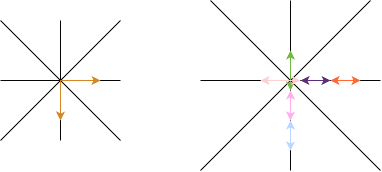
\includegraphics{Figure1.drawio.png}\\

Where the brown line is OPT with a single path. And Green Pink Light blue take over 1 line and orange purple light pink take over the other. Note that an important part which is omitted here is that Brown doesn't have to be $2^i$ len on every line causing us to gain more paths in OPT in that case. which is at most 1 more per line.\\\\
Now we will use the Classify And Randomly Select algorithm (with the greedy one). and since we have exactly $\log 2n$ different groups since the largest size is $2n$ we have a competitiveness of $6\log 2n$ which is $O(\log n)$ as requested.